% The entire content of this work (including the source code
% for TeX files and the generated PDF documents) by 
% Hongxiang Chen (nicknamed we.taper, or just Taper) is
% licensed under a 
% Creative Commons Attribution-NonCommercial-ShareAlike 4.0 
% International License (Link to the complete license text:
% http://creativecommons.org/licenses/by-nc-sa/4.0/).
\documentclass{article}

% My own physics package
% The following line load the package xparse with additional option to
% prevent the annoying warnings, which are caused by the package
% "physics" loaded in package "physicist-taper".
\usepackage[log-declarations=false]{xparse}
\usepackage{physicist-taper}
\makenomenclature % For an index of symbols.

\title{Condensed Matter Field Theory notes}
\date{\today}
\author{Taper}


\begin{document}


\maketitle
\abstract{
Notes of book \cite{Altland2010}, and another book \cite{Greiner1996} for
information about path integral.
}
\tableofcontents

\section{Todo}

\begin{enumerate}
    \item Understand in what case can the Gaussian integral formula can be
        applied. In another word, understand the analytical continuation of the
        Gaussian integral. See for example, buttom of pp.343 of
        \cite{Greiner1996}.
        \label{todo:analytical-c}
    \item Understand the Wick Rotation, cf. pp.356(ch11.5) of
        \cite{Greiner1996}. This is related to todo \ref{todo:analytical-c}
    \item Understand how the constant term in the path integral of a Feynman
        Kernal will(or will not) affect the physics. Understand the mathematical
        rationale to support this. (cf. buttom of pp.344 of \cite{Greiner1996}.
    \item I have doubt about the correctness of pp.110 eq 3.28 till pp.111
        (Construction recipe of the path integral), especially about his
        argument, the size of the \textit{Planck cell}.
\end{enumerate}

Bonus objectives:
\begin{enumerate}
    \item Find abou the similarity between Path Integral of a free particle and
        the solution to a classical diffusion equation (cf. pp.112, footnote 1
        of \cite{Altland2010}).
    \item Those marked \textit{todo} in \cite{Altland2010}.
\end{enumerate}
\section{pp.33 eq.1.43}
\label{sec:Table}

In page 33 of \cite{Altland2010}, the author derives a difference of action, when we
have a symmetry transformation paraterized by $\omega_a$:

\begin{align}
    x_\mu \to x'_\mu &= x_\mu + \frac{\partial x_\mu}{\omega_a}|_{\omega=0} \omega_a(x) \\
    \phi^i(x) \to \phi'(x') &= \phi^i(x) + \omega_a(x)F^i_a[\phi]
\end{align}

We have:
\begin{align}
    \mathcal{L} &= \mathcal{L}(\phi^i(x),\partial_{x_\mu}\phi^i(x)) \\
    \mathcal{L}' &= \mathcal{L'}(\phi'^i(x'),\partial_{x'_\mu}\phi'^i(x')) \\
    &= \mathcal{L}\left(\phi^i+F^i_a\omega_a, 
                    \left(\delta_{\mu\nu}-\partial_{x_\mu}(\omega_a
                    \partial_{\omega_a}x_\mu)\right)
                    \partial_{x_\nu}(\phi^i+F^i_a\omega_a)
                  \right)
\end{align}
And 

\begin{align}
    \Delta S &= \int \dd[m]{x'} \mathcal{L}' - \int \dd[m]{x} \mathcal{L} 
    \label{eq:dS-integrand}\\
    &=
    \int \dd[m]{x}
    \left(1+\partial_{x_\mu}\left(\omega_a \partial_{\omega_a}x_\mu\right) \right) 
    \nonumber\\
    &\times \mathcal{L}\left(
                    \phi^i+F^i_a\omega_a, 
                    \left(\delta_{\mu\nu}-\partial_{x_\mu}\left(\omega_a
                        \partial_{\omega_a}x_\mu\right)\right)
                        \partial_{x_\nu}(\phi^i+F^i_a\omega_a)
                    \right) \nonumber\\
    &- \int \dd[m]{x}  \mathcal{L}(\phi^i(x),\partial_{x_\mu}\phi^i(x))
\end{align}

Then he argues that, "for constant parameters $\omega_a$ the action difference
$\Delta a$ vanishes". Therefore "the leading contribution to the action
difference of a symmetry transformation must be linear in the derivative
$\partial_{x_\mu}\omega_a$".

Then he writes that "A straightforward expansion of the formula above
for $\Delta S$ shows that these terms are given by"

\begin{equation}
    \Delta S = -\int \dd[m]{x} j^a_\mu (x) \partial_{x_\mu}\omega_a
\end{equation}
where $j^a_\mu$ is:
\begin{equation}
    j^a_\mu = \left(
        \frac{\partial \mathcal{L}}{\partial(\partial_{x_\mu}\phi^i)}
            \partial_{x_\nu}\phi^i
        -\mathcal{L}\delta_{\mu\nu} \right) \frac{\partial x_\nu}{\partial\omega_a}
    - \frac{\partial\mathcal{L}}{\partial(\partial_{x_\mu}\phi^i)} F^i_a
\end{equation}

I am partically confused about how to do the "straightforward expansion". I
guess I should do $\frac{\partial}{\partial (\partial_{x_\mu}\omega_a)}$ to the
integrand inside expression for $\Delta S$, though I don't really understand the
reason. Even so, the integrand contains terms like
$\partial_{x_\mu}\partial_{\omega_a}x_\mu$, which I don't know how to deal with.

\textbf{Solution}. The reality is a bit more complicated. We first do a first
order expasion to get the infinitesimal difference:

\begin{align}
    &\mathcal{L}'-\mathcal{L} \\
    \approx &
    \frac{\partial \mathcal{L}}{\partial\phi^i} F^i_a\omega_a
    +\frac{\partial \mathcal{L}}{\partial(\partial_{x_\mu}\phi^i)}
        \left[
        \partial_\mu\left(F^i_a\omega_a\right) 
            - \partial_\mu\left(\omega_a\frac{\partial x_\nu}{\partial\omega_a}\right)
                \partial_\nu\left(\phi^i+F^i_a\omega_a\right)
        \right]
    \nonumber\\
    =&\quad
    \omega_a
    \left[
        \frac{\partial \mathcal{L}}{\partial\phi^i}F^i_a 
        +
        \frac{\partial \mathcal{L}}{\partial(\partial_{x_\mu}\phi^i)}
        \left(
            \partial_\mu F^i_a 
            - \partial_\mu(\frac{\partial x_\nu}{\partial \omega_a})
            \partial_\nu(\phi^i+F^i_a\omega_a)
        \right)
    \right]
    \label{eq:l-l-omega}
    \\
    +&
    \partial_\mu\omega_a
    \left[
        \frac{\partial \mathcal{L}}{\partial(\partial_{x_\mu}\phi^i)}
        \left(
            F^i_a-\frac{\partial x_\nu}{\partial \omega_a}
            \partial_\nu(\phi^i+F^i_a\omega_a)
        \right)
    \right]
    \label{eq:l-l-pmu-omega}
\end{align}

We also discover the integrand in Eq.\ref{eq:dS-integrand} to be
\begin{align}
    &\left(1+\partial_\mu(
        \omega_a\frac{\partial x_\mu}{\partial \omega_a})
        \right)\mathcal{L}'-\mathcal{L} 
    \\
    =& 
    \left(
    1+\partial_\mu(\omega_a\frac{\partial x_\mu}{\partial \omega_a})
    \right)
    (\mathcal{L}'-\mathcal{L})
    +
    \left(\partial_\mu(\omega_a\frac{\partial x_\mu}{\partial \omega_a})\right)
    \mathcal{L}
    \label{eq:integrand-l-density}
\end{align}
For the first term 
$\left(
    1+\partial_\mu(\omega_a\frac{\partial x_\mu}{\partial \omega_a})
\right) (\mathcal{L}'-\mathcal{L}) $, the $(\mathcal{L}'-\mathcal{L})$ already
has terms of first order of $\omega_a$ and of first order of
$\partial_\nu\omega_a$. For our purpose, the second order terms
($\partial_\nu(F^i_a\omega_a)$) from item \ref{eq:l-l-omega} and item
\ref{eq:l-l-pmu-omega} can be ignored. Also, the item
$(\partial_\mu(\omega_a\frac{\partial x_\mu}{\partial
\omega_a}))(\mathcal{L}'-\mathcal{L})$ in eq.\ref{eq:integrand-l-density} can
also be ignored.

Therefore the integrand in Eq.$\ref{eq:dS-integrand}$ becomes

\begin{align}
    & (\mathcal{L}'-\mathcal{L})
    +
    \left(\partial_\mu(\omega_a\frac{\partial x_\mu}{\partial \omega_a})\right)
    \mathcal{L} \\
    = & 
    \omega_a
    \left[
        \frac{\partial \mathcal{L}}{\partial\phi^i}F^i_a 
        +
        \frac{\partial \mathcal{L}}{\partial(\partial_{x_\mu}\phi^i)}
        \left(
            \partial_\mu F^i_a 
            - (\partial_\mu\frac{\partial x_\nu}{\partial \omega_a})
            \partial_\nu(\phi^i+F^i_a\omega_a)
        \right)
        +
        (\partial_\nu \frac{\partial x_\mu}{\partial \omega_a})\mathcal{L}
    \right]
    \\
    +&
    \partial_\mu\omega_a
    \left[
        \frac{\partial \mathcal{L}}{\partial(\partial_{x_\mu}\phi^i)}
        \left(
            F^i_a-\frac{\partial x_\nu}{\partial \omega_a}
            \partial_\nu(\phi^i+F^i_a\omega_a)
        \right)
        +
        \frac{\partial x_\mu}{\partial \omega_a}\mathcal{L}
    \right]
\end{align}

Therefore, the term we seek, i.e. the coefficient of $\partial_\mu\omega_a$ is
\begin{align}
  & \frac{\partial \mathcal{L}}{\partial(\partial_{x_\mu}\phi^i)}
    \left(
        F^i_a-\frac{\partial x_\nu}{\partial \omega_a}
        \partial_\nu(\phi^i+F^i_a\omega_a)
    \right)
    +
    \frac{\partial x_\mu}{\partial \omega_a}\mathcal{L} \\
    =&
    \left(
        \mathcal{L}\delta_{\mu\nu}
        -\frac{\partial \mathcal{L}}{\partial(\partial_{x_\mu}\phi^i)}
            \partial_\nu \phi^i
    \right) \frac{\partial x_\nu}{\partial \omega_a}
    +
    \frac{\partial \mathcal{L}}{\partial(\partial_{x_\mu}\phi^i)}F^i_a
\end{align}
which is what we expect in equation 1.43 of \cite{Altland2010}.

\textbf{Question}: as for why we should ignore the term with $\omega_a$, there
are two posts (
    \href{http://physics.stackexchange.com/questions/122965/derivation-of-the-noether-current}{[1]},
    \href{http://physics.stackexchange.com/questions/99853/on-a-trick-to-derive-the-noether-current}{[2]} )
might be useful for a thought.

\todo{confusion}

I had great doubt about this problem. Though I have posted an answer on
\href{http://physics.stackexchange.com/questions/122965/derivation-of-the-noether-current}{[1]},
I don't think that answer is satisfactory.

\section{About \texorpdfstring{$\dot{q}$}{} and imaginary time}

The $\dot{q}$ in all the path integrals, especially eq.3.6 and eq.3.8, is in
fact a shorthand for the divided difference $\frac{q_{n+1}-q_n}{\Delta t}$ as in
pp.99 (the buttom). It is not exactly the same as $\dot{q}$. pp.343 of
\cite{Greiner1996} also mentioned that in this sense, the Lagrangian in all
path integrals is not identical with the ordinary Lagrange function. Though, I
still do not know if this matters at all.

In the most common imaginary time transformation, such as those mentioned in
pp.106 of \cite{Altland2010}, and pp.358 of \cite{Greiner1996}, we have the
transformation $t\to -i\tau$. This in effect change all the $\Delta t$ in, e.g.
eq 3.5 (pp.99) of \cite{Altland2010}, to $-i\Delta\tau$. Therefore, the divided
difference
$$ \frac{q_{n+1}-q_n}{\Delta t} \to \frac{q_{n+1}-q_n}{-i \Delta\tau}$$
Therefore,
$$ \dot{q} \to i\partial_\tau q $$
$$ \dot{q}^2 \to -\partial^2_\tau q $$
\section{Eq. 3.5}

It is not so obvious to get Eq.3.5 in pp.99 of \cite{Altland2010}. Here is my
notes.

According to the book, Eq.3.3 is turned into (I set $\hbar=1$ occasionally,
though sometimes I forgot that I have set $\hbar=1$, orz):
\begin{align}
    \bra{q_f} 
    &\int \dd{q_N}\dd{p_N}\ket{q_N}\braket{q_N|p_N}\bra{p_N}
        e^{-i\hat{T}\Delta t}e^{-i\hat{V}\Delta t}\times \nonumber\\
    &   \int \dd{q_{N-1}}\dd{p_{N-1}}\ket{q_{N-1}}\braket{q_{N-1}|p_{N-1}}\bra{p_{N-1}}
        e^{-i\hat{T}\Delta t}e^{-i\hat{V}\Delta t} \times
        \dots \nonumber\\
    &   \int \dd{q_1}\dd{p_1}\ket{q_1}\braket{q_1|p_1}\bra{p_1}
        e^{-i\hat{T}\Delta t}e^{-i\hat{V}\Delta t} \ket{q_i}
\end{align}
Notice that
\todo{T has only p, V has only q}
\begin{align}
    \braket{q|p} &= \frac{\exp(iqp/\hbar)}{\sqrt{2\pi\hbar}} \\
    \bra{p_N}e^{-i\hat{T}\Delta t} &= \bra{p_N}e^{-iT(p_N)\Delta t} \\
    e^{-i\hat{V}\Delta t}\ket{q_{N-1}} &= e^{-iV(q_{N-1})\Delta t}\ket{q_{N-1}} \\
\end{align}
Also, 
\begin{align}
    &\braket{q_N|p_N}\bra{p_N}e^{-i\hat{T}\Delta t}e^{-i\hat{V}\Delta t}\ket{q_{N-1}} 
    = \frac{e^{iq_N p_N/\hbar}}{\sqrt{2\pi\hbar}}
        \bra{p_N}e^{-iT(p_N)\Delta t} e^{-iV(q_{N-1})\Delta t}\ket{q_{N-1}}
    \nonumber\\
    =& \frac{e^{iq_N p_N/\hbar}}{\sqrt{2\pi\hbar}}
        \braket{p_N | q_{N-1}}e^{-iT(p_N)\Delta t} e^{-iV(q_{N-1})\Delta t}
    = \frac{e^{ip_N (q_N-q_{N-1})/\hbar}}{2\pi\hbar}
        e^{-i[T(p_N)+V(q_{N-1})]\Delta t} 
\end{align}
etc. Now we have to pay special attentiont to the start and end. For the start,
we have a
$$ \int \dd{q_N} \braket{q_f | q_N} = \int\dd{q_N}\delta(q_N-q_f) $$
So every $q_N$ is replaced by $q_f$. For the end, we have
$$ \braket{q_1|p_1}\bra{p_1}e^{-i\hat{T}\Delta t}e^{-i\hat{V}\Delta t} \ket{q_i}
= e^{-i[T(p_1)+V(q_i)]}\frac{e^{ip_1(q_1-q_i)}}{2\pi\hbar}
$$

Together we have the whole thing into:

\begin{align}
    \int & \dd{q_1}\cdots\dd{q_{N-1}}\dd{p_1}\dd{p_N} \frac{1}{(2\pi\hbar)^N}
    \times \nonumber\\
  & e^{i\left[p_1(q_1-q_i)+\cdots p_N(q_N-q_{N-1})\right]} \times\nonumber\\
  & e^{-i\left[T(p_1)+\cdots+T(p_N)+V(q_i)+V(q_1)+\cdots+V(q_{N-1})\right]}
\end{align}
which is exactly eq.(3.5) in book.
\section{Eq 9.4}

The Hamiltonian for particle on a ring is claimed to be (Eq. 9.1 of
\cite{Altland2010}, pp. 498):
\begin{equation}
    H = \frac{1}{2}(-i\partial_\phi -A)^2 = \frac{1}{2}(p-A)^2
\end{equation}

The book \cite{Altland2010} claims that 
\begin{equation}
    L = \frac{1}{2}\dot{\phi}^2 - iA \dot{\phi}
\end{equation}
I am quite confused, especially about the appearance of $\dot{\phi}$. Can any explain
a bit?

How I tried: Since the inverse of a Legendre transformation is Legendre
transformation itself, 
\begin{align}
    \text{Denote }x &\equiv \frac{\partial H}{\partial p} = p-A,\text{ so,} \\
    p &= x + A,\quad H = \frac{1}{2}x^2 ,\text{ so,}\\
    L = x p - H &= x(x+A) - \frac{1}{2}x^2 = \frac{1}{2}x^2 + x A 
\end{align}
So my calculation found that the Lagrangian of above Hamiltonian is:
\begin{equation}
    L = \frac{1}{2}x^2 + x A
\end{equation}
where
\begin{equation}
    x = \frac{\partial H}{\partial p}
\end{equation}


\bibliography{cite}{}
\bibliographystyle{alphaurl}

\printnomenclature
\section{A brief Summary of Quantum double well}

The Quantum double well:
\begin{figure}[H]
    \centering
    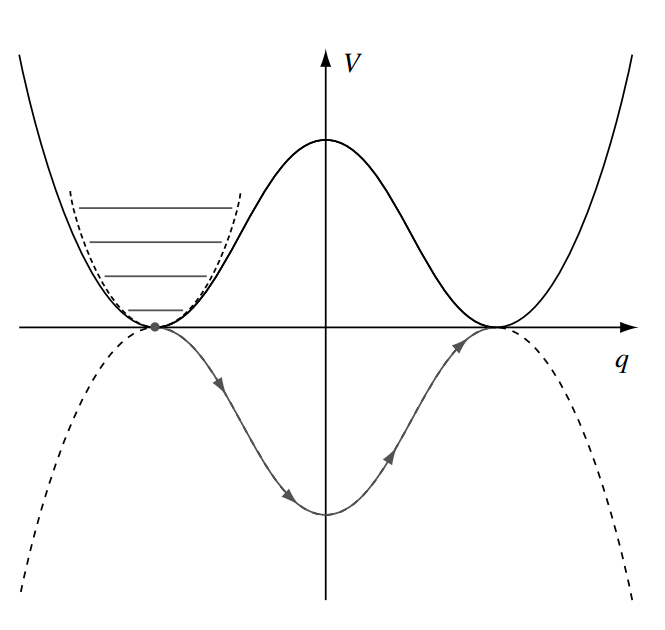
\includegraphics[width=0.6\linewidth]{pics/quantum-double-well.png}
    \caption{Quantum double well}
    The solid line is the double well potential. The dotted line in
    the second quarter is to remind us of the single well potential and its sets
    of eigenvalues. The inverted potential in Euclidean time is shown below the
    $q$-axis.
\end{figure}
The Euclidean path integral is
\begin{equation}
    G_E(a,\pm a:\tau)=\int_{q(0)=\pm a,q(\tau)=a} Dq\,
    \exp(-\frac{1}{\hbar}\int_0^\tau\dd{\tau'}
        \left(\frac{m}{2}\dot{q}^2+V(q)\right)
    )
\end{equation}
with the imaginary time saddle point equation
\begin{equation}
    -m\ddot{q}+V'(q) = 0
\end{equation}

It is turned into several contributions:
\begin{equation}
    A = A_{cl}\times A_{qu}
\end{equation}
where $A$ denotes transition amplitude, "cl" for classical, "qu" for quantum.

The classical contribution includes a stationary not moving part $A_{cl,st}$, a
moving but bouncing back and forth in the inverted potential part $A_{cl,inst}$.
The moving and bouncing back and forth motion is termed \nomen{instanton}, see
p.117(\cite{Altland2010}) for details.

The $A_{cl,st}$ is $e^{0}=1$ since the stationary path $q\equiv0$. The
$A_{cl,inst}$ is calculated in the book (pp.116-117), and the result is:
\begin{equation}
    A_{cl,inst,one-trip} = \exp(-\frac{1}{\hbar}S_{inst})
\end{equation}
for one bouncing trip. Here $S_{inst}$ is given by eq.3.36 in p.117. Adding them
together gives:
\begin{equation}
    A_{cl,inst} =
    \sum_{n\text{ even/odd}}^\infty \frac{1}{n!}
    \left(\tau K e^{-S_{inst}/\hbar}\right)^n
    =\cosh(\tau Ke^{-S_{inst}/\hbar})\text{ or }\sinh(\tau Ke^{-S_{inst}/\hbar})
\end{equation}

where $K$ is just some prefactor explained in p.118 and calculated in
pp.122-123.

The quantum contribution is due to the fluctuation of path around the classical
path. This part is also divided into two categories. The $A_{qu,st}$ for
fluctuation around the stationary path is calculated in the section about single
well green function, spcifically eq.3.31 in p.114. It is approximated in p.119
to be
\begin{equation}
    A_{qu,st,n} = e^{-\omega(\tau_{i+1}-\tau_i)/2}
\end{equation}
and adding together gives
\begin{equation}
    A_{qu,st}= \prod_i e^{-\omega(\tau_{i+1}-\tau_i)/2} = e^{-\tau\omega}
\end{equation}
The rest $A_{qu,inst}$ from fluctuation around instanton is assumed to be
negligible (p.119).

In summary:
\begin{table}[H]
    \centering
    \begin{tabular}{l c c}
        Path       & Classical ($0$th order) & Fluctuation ($2$nd order) \\
        Stationary & $1$                     & $\approx e^{-\omega\tau}$  \\
        Instanton  & $e^{-\frac{1}{\hbar}S_{\text{inst}}}$, or $\cosh(\tau Ke^{-S_{\text{inst}}/\hbar}) \sinh(\tau Ke^{-S_{\text{inst}}/\hbar})$ & $\approx 1$\\
    \end{tabular}
\end{table}

\section{License}
The entire content of this work (including the source code
for TeX files and the generated PDF documents) by 
Hongxiang Chen (nicknamed we.taper, or just Taper) is
licensed under a 
\href{http://creativecommons.org/licenses/by-nc-sa/4.0/}{Creative 
Commons Attribution-NonCommercial-ShareAlike 4.0 International 
License}. Permissions beyond the scope of this 
license may be available at \url{mailto:we.taper[at]gmail[dot]com}.
\end{document}
